%HW3.tex
%
% Third Homework for Graduate Algebra
% Frank Sottile
%%%%%%%%%%%%%%%%%%%%%%%%%%%%%%%%%%%%%%%%%%%%%%%%%%%%%%%%%%%%%%%%%%%%%%%
\documentclass[12pt]{article}
\usepackage{multicol,amssymb,amsmath}
\usepackage{graphicx}
\usepackage{xcolor}
\headheight=8pt
%
\topmargin=-95pt
\textheight=744pt   \textwidth=575pt
\oddsidemargin=-60pt \evensidemargin=-60pt

\pagestyle{empty}

%%%%%%%%%%%%%%%%%%%%%%%%%%%%%%%%%%%%%%%%%%%%
\newcommand{\HH}{{\mathbb H}}
\newcommand{\FF}{{\mathbb F}}
\newcommand{\RR}{{\mathbb R}}
\newcommand{\CC}{{\mathbb C}}
\newcommand{\KK}{{\mathbb K}}
\newcommand{\NN}{{\mathbb N}}
\newcommand{\TT}{{\mathbb T}}
\newcommand{\ZZ}{{\mathbb Z}}
\newcommand{\calA}{{\mathcal A}}
\newcommand{\be}{{\bf e}}

\newcommand{\Hom}{\mbox{Hom}}
\newcommand{\End}{\mbox{End}}
\newcommand{\Mat}{\mbox{Mat}}
\newcommand{\rank}{\mbox{rank}}
\newcommand{\spec}{\mbox{spec}}
\newcommand{\cone}{\mbox{cone}}

\newcommand{\Square}{\raisebox{-2pt}{\includegraphics{figures/Square.eps}}}

\newcommand{\vect}[2]{(\begin{smallmatrix}#1\\#2\end{smallmatrix})}
\newcommand{\msp}{\hspace{8pt}}

\newcommand{\barsl}{\noindent\begin{minipage}[t]{575pt}
{\color{violet}\rule{575pt}{1.2pt}}\vspace{-5.7mm}\\
{\color{blue}\rule{575pt}{1.2pt}}\vspace{-5.7mm}\\
{\color{green}\rule{575pt}{1.2pt}}\vspace{-5.7mm}\\
{\color{yellow}\rule{575pt}{1.2pt}}\vspace{-5.7mm}\\
{\color{orange}\rule{575pt}{1.2pt}}\vspace{-5.7mm}\\
{\color{red}\rule{575pt}{1.2pt}}
\end{minipage}}


\def\demph#1{{\color{blue}{\sl #1}}}
\def\defcolor#1{{\color{blue}#1}}

\begin{document}
\LARGE 
\noindent
Algebra II\ \ Winter 2021 \hfill 1 February\makebox[40pt][l]{\ }\\
Frank Sottile \hfill
\Large\sf
Third Homework\makebox[40pt][l]{\ }\\
%\large\vspace{5pt}
\normalsize

\noindent
Write your answers neatly, in complete sentences, and prove all assertions.
Start each problem on a new page (this makes it easier in Gradescope).
Revise your work before handing it in, and submit a .pdf  created from a LaTeX source to Gradescope.
Correct and crisp proofs are greatly appreciated; oftentimes your work can be shortened and made clearer.

{\color{red}Due Monday 8 February.}\vspace{-5pt}\newline

\barsl

\begin{enumerate}
%%%%%%%%%%%%%%%%%%%%%%%%%%%%%%%%%%%%%
%\setcounter{enumi}{52}


%\newpage
%%%%%%%%%%%%%%%%%%%%%%%%%%%%%%%%%%%%%%%%%%%%%%%%%%%%%%%%%%%%%%%%%%%%%%%%%%%%%%%%%
\item  Let $V$ be a finite-dimensional vector space over a field $\FF$.
  The set \defcolor{$\End_{\FF}(V)$} of linear transformations $T\colon V\to V$ of $V$ forms a ring with multiplication the composition of maps.
  (If $n=\dim_\FF(V)$, then $\End_\FF(V)\simeq\Mat_{n\times n}(\FF)$, given by any ordered basis of $V$.)
  Verify that $V$ is naturally an  $\End_{\FF}(V)$-module and identify its submodules.
 \vspace{-2pt}
%%%%%%%%%%%%%%%%%%%%%%%%%%%%%%%%%%%%%%%%%%%%%%%%%%%%%%%%%%%%%%%%%%%%%%%%%%%%%%%%%

%\newpage
%%%%%%%%%%%%%%%%%%%%%%%%%%%%%%%%%%%%%%%%%%%%%%%%%%%%%%%%%%%%%%%%%%%%%%%%%%%%%%%%%
\item Let $\FF$ be a field, $V$ a finite-dimensional vector space over $\FF$, and $T\colon V\to V$ a linear transformation.
  
  Show that the ring homomorphism induced by $x\mapsto T$ equips $V$ with the structure of a module over the polynomial ring $\FF[x]$.

  What are the $\FF[x]$-submodules of $V$ under this action ?      
 \vspace{-2pt} 
%%%%%%%%%%%%%%%%%%%%%%%%%%%%%%%%%%%%%%%%%%%%%%%%%%%%%%%%%%%%%%%%%%%%%%%%%%%%%%%%%


%\newpage
%%%%%%%%%%%%%%%%%%%%%%%%%%%%%%%%%%%%%%%%%%%%%%%%%%%%%%%%%%%%%%%%%%%%%%%%%%%%%%%%%
 \item   Suppose that $\phi\colon M\to N$ and $\psi\colon N\to M$ are $R$-module homomorphisms
   such that $\psi\circ\phi=1_M$ (the identity map on $M$).
   Prove that $N=\mbox{\rm image}(\phi) \oplus\mbox{\rm kernel}(\psi)$.
   \vspace{-2pt}
%%%%%%%%%%%%%%%%%%%%%%%%%%%%%%%%%%%%%%%%%%%%%%%%%%%%%%%%%%%%%%%%%%%%%%%%%%%%%%%%%

%\newpage
%%%%%%%%%%%%%%%%%%%%%%%%%%%%%%%%%%%%%%%%%%%%%%%%%%%%%%%%%%%%%%%%%%%%%%%%%%%%%%%%%
 \item Suppose that $R$ is a principal ideal domain, $A$ a left $R$-module, and $p\in R$ a prime (and hence also irreducible).
   Recall that $R/pR$ is a field.
   
   Show that both $\defcolor{pA}:=\{pa\mid a\in A\}$ and $\defcolor{A[p]}:=\{a\in A\mid pa=0\}$ are $R$-submodules of $A$.

   Show that $A/pA$ and $A[p]$ are both  naturally vector spaces over $R/pR$.
   (Part of this is interpreting 'naturally', but there is only one sensible choice of the action.)
   \vspace{-2pt}
%%%%%%%%%%%%%%%%%%%%%%%%%%%%%%%%%%%%%%%%%%%%%%%%%%%%%%%%%%%%%%%%%%%%%%%%%%%%%%%%%

%\newpage
%%%%%%%%%%%%%%%%%%%%%%%%%%%%%%%%%%%%%%%%%%%%%%%%%%%%%%%%%%%%%%%%%%%%%%%%%%%%%%%%%
 \item Let $V$ be a vector space over a division ring $D$ and $S$ the set of all subspaces of $V$, partially ordered by inclusion.

   Show that $S$ is a \demph{complete lattice} (defined in Exercise 7.2 of the Introdution to Hungerford) with least upper bound of $U,W$
   equal to $U+W$ and greatest lower bound $U\cap W$.

   Show that $S$ is \demph{complemented}; for all $W\in S$, there is a $U\in S$ such that $W+U=V$ and $W\cap U=\{0\}$.

   Show that $S$ is \demph{modular}; for $A,B,C\in S$ with $C\subset A$, we have $A\cap(B+C)=(A\cap B)+C$.
   \vspace{-2pt}
%%%%%%%%%%%%%%%%%%%%%%%%%%%%%%%%%%%%%%%%%%%%%%%%%%%%%%%%%%%%%%%%%%%%%%%%%%%%%%%%%


%\newpage
%%%%%%%%%%%%%%%%%%%%%%%%%%%%%%%%%%%%%%%%%%%%%%%%%%%%%%%%%%%%%%%%%%%%%%%%%%%%%%%%%
 \item If $F$ and $G$ are free modules over a ring with the invariant dimension property, show that\newline 
   $\rank(F\oplus G)=\rank(F)+ \rank(G)$.
   \vspace{-2pt}
%%%%%%%%%%%%%%%%%%%%%%%%%%%%%%%%%%%%%%%%%%%%%%%%%%%%%%%%%%%%%%%%%%%%%%%%%%%%%%%%%

%\newpage
%%%%%%%%%%%%%%%%%%%%%%%%%%%%%%%%%%%%%%%%%%%%%%%%%%%%%%%%%%%%%%%%%%%%%%%%%%%%%%%%%
 \item Let $R$ be a ring with no zero divisors such that for all $r,s\in R$, there are $a,b\in R$, not both zero, such that $ar+bs=0$.
   Show that if $R=M\oplus N$ as $R$-modules, then one of $M$ or $N$ is the 0-module, $\{0\}$.
   Use this to show that $R$ has the invariant dimension property. 
   \vspace{-2pt}
%%%%%%%%%%%%%%%%%%%%%%%%%%%%%%%%%%%%%%%%%%%%%%%%%%%%%%%%%%%%%%%%%%%%%%%%%%%%%%%%%

%\newpage
%%%%%%%%%%%%%%%%%%%%%%%%%%%%%%%%%%%%%%%%%%%%%%%%%%%%%%%%%%%%%%%%%%%%%%%%%%%%%%%%%
 \item Show that if $F$ is a free module over a ring $R$ such that $F$ has a basis of cardinality an integer
   $n\geq 1$, and {\sl another} basis  with cardinality $n{+}1$, then $F$ has a basis of every cardinality $m\in \NN$ with $m\geq n$.

   Note that the ring $R$ is necessarily noncommutative.
   \vspace{-2pt}
%%%%%%%%%%%%%%%%%%%%%%%%%%%%%%%%%%%%%%%%%%%%%%%%%%%%%%%%%%%%%%%%%%%%%%%%%%%%%%%%%

\end{enumerate}
%%%%%%%%%%%%%%%%%%%%%%%%%%%%%%%%%%%%%%%%%%%%%%%%%%%%%%%%%%%%%%%


\end{document}

%\newpage
%%%%%%%%%%%%%%%%%%%%%%%%%%%%%%%%%%%%%%%%%%%%%%%%%%%%%%%%%%%%%%%%%%%%%%%%%%%%%%%%%
\item 
   \vspace{-2pt}
%%%%%%%%%%%%%%%%%%%%%%%%%%%%%%%%%%%%%%%%%%%%%%%%%%%%%%%%%%%%%%%%%%%%%%%%%%%%%%%%%
